\documentclass[12pt,a4paper]{article}
\usepackage[UTF8]{ctex}
\usepackage{geometry}
\geometry{left=2.5cm,right=2.5cm,top=2.5cm,bottom=2.5cm}
\usepackage{graphicx}
\usepackage{booktabs}
\usepackage{hyperref}
\usepackage{amsmath}
\usepackage{caption}

\title{Origami Hand CAD 编辑器：折纸手图形化设计工具}
\author{论文附录}
\date{}

\begin{document}
\maketitle

\section{概述}

Origami Hand CAD 编辑器是本论文折纸手设计流程的核心入口工具。该工具基于 PyQt5 图形界面框架开发，提供了一个完整的二维图形化设计环境。用户无需编写任何代码，即可通过鼠标交互完成从折痕线绘制到腱绳路径定义的全部设计工作。

\section{功能模块}

CAD 编辑器的工具栏包含以下绘图模式：

\begin{itemize}
    \item \textbf{轮廓线（L 键）}：绘制折纸手的外形轮廓，作为面片分割的边界。
    \item \textbf{峰折线（M 键）}：绘制凸向观察者的折痕（Mountain fold），用红色实线表示。峰折在几何折叠后产生负向关节角。
    \item \textbf{谷折线（V 键）}：绘制凹向观察者的折痕（Valley fold），用蓝色实线表示。谷折产生正向关节角。
    \item \textbf{滑轮（P 键）}：在折痕上放置导向滑轮，指定半径 $r$ 和摩擦系数 $\mu$。滑轮通过啮合于折痕线来施加驱动力矩。
    \item \textbf{孔（H 键）}：在面片上放置孔类导向元件，指定板厚偏移 $h$ 和摩擦系数 $\mu$。孔通过跨折痕的腱绳张力产生驱动力矩。
    \item \textbf{腱绳（T 键）}：依次点击滑轮、孔和驱动器定义腱绳路径。程序自动维护元素 ID 序列。
    \item \textbf{驱动器（A 键）}：放置两台驱动器 Motor A 和 Motor B，作为腱绳两端的驱动源。
    \item \textbf{阻尼器（D 键）}：放置粘滞阻尼器（用于扩展的动态协同模型，本文 SDAS 模型不使用）。
\end{itemize}

\section{设计文件格式}

完成设计后，用户通过``文件 $\to$ 保存 .ohd'' 将全部几何和拓扑信息保存为 JSON 格式的 \texttt{.ohd} 文件。该文件包含折痕线坐标、折痕类型和刚度、滑轮/孔/阻尼器参数、腱绳元素 ID 序列以及驱动器位置等所有设计信息。\texttt{.ohd} 文件是连接 CAD 设计与后续仿真流程（传动计算、SDAS 协同求解、MuJoCo 交互仿真）的桥梁。

\section{设计案例}

图\,\ref{fig:cad_screenshot} 展示了一个典型的三指折纸手设计（ohd\_6）在 CAD 编辑器中的二维视图。该设计包含 36 条折痕线、42 个导向滑轮、2 台驱动器和 1 条腱绳。图中红色实线为峰折，蓝色实线为谷折，灰色虚线为轮廓线。绿色圆点为滑轮，紫色折线为腱绳路径，红色与蓝色矩形分别为驱动器 A 和驱动器 B。

\begin{figure}[htbp]
    \centering
    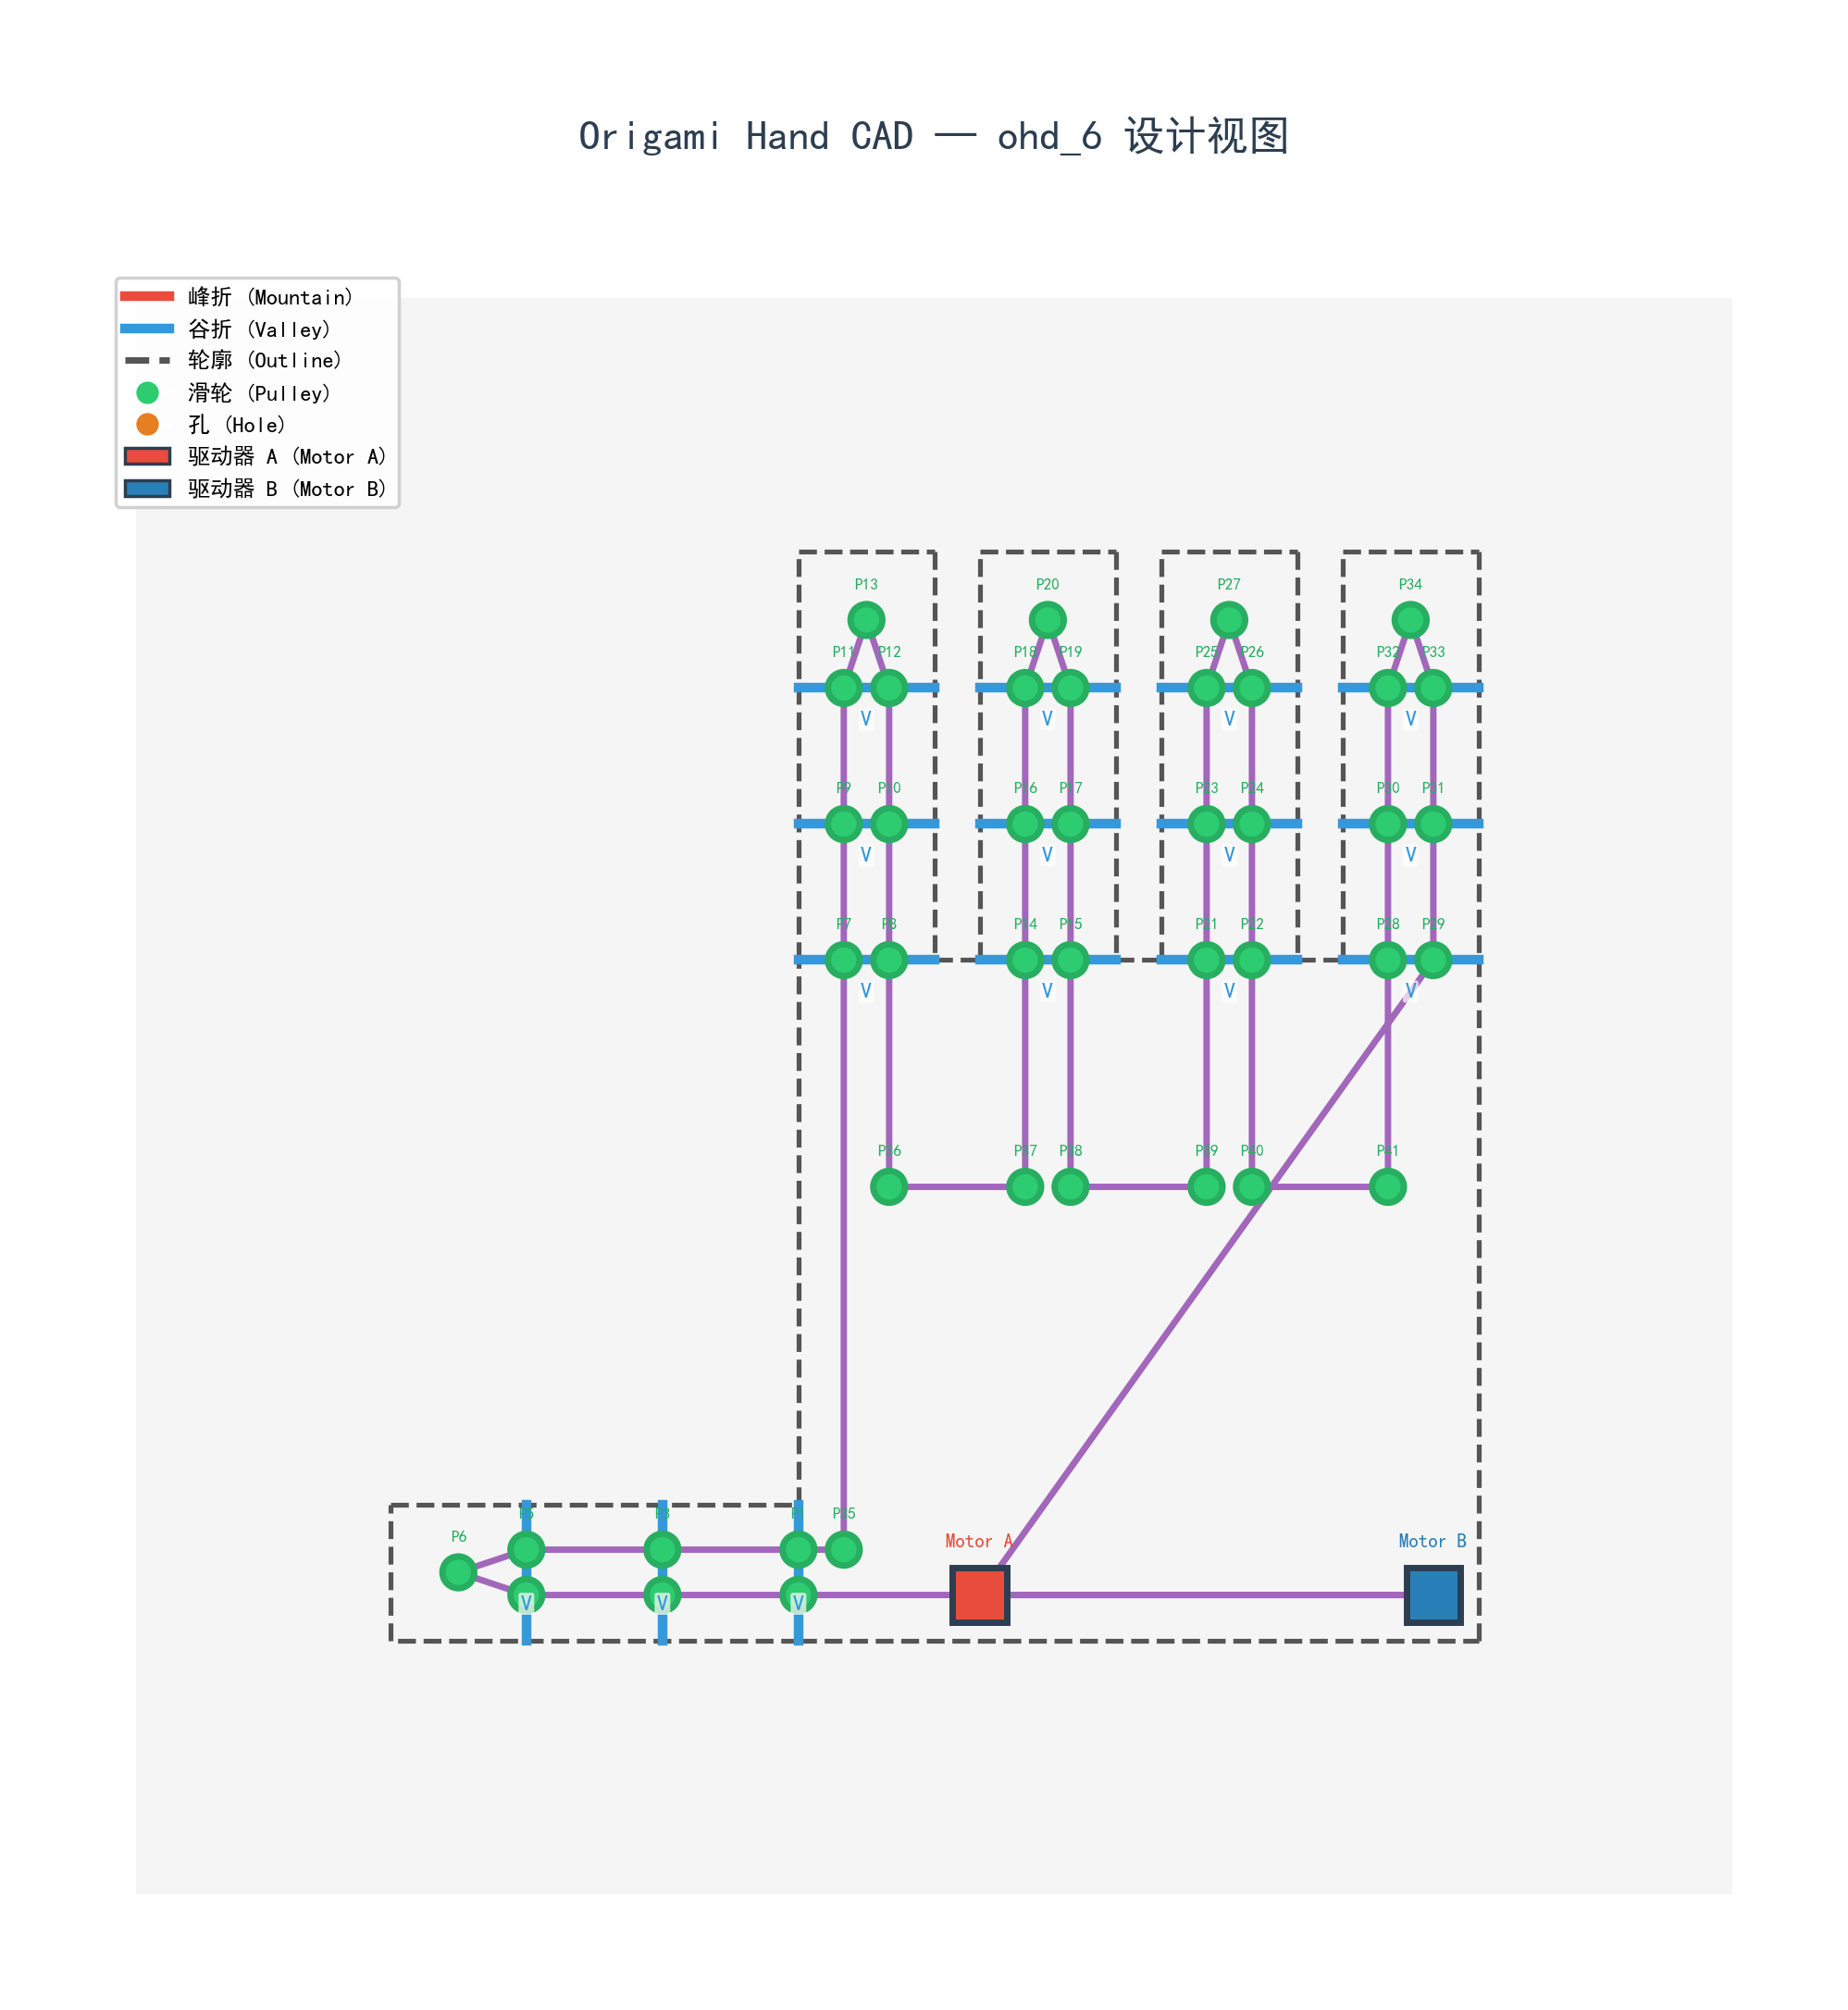
\includegraphics[width=0.95\textwidth]{figures/cad_ohd6_screenshot.png}
    \caption{Origami Hand CAD 编辑器界面（ohd\_6 三指折纸手设计）。红色实线：峰折；蓝色实线：谷折；灰色虚线：轮廓；绿色圆点：滑轮；紫色折线：腱绳路径；红色/蓝色方块：驱动器 A/B。右侧属性面板可调整选中元素的参数。}
    \label{fig:cad_screenshot}
\end{figure}

图\,\ref{fig:cad_screenshot} 可以清晰地看到折纸手的骨架结构：三根手指呈放射状分布，每根手指由多条折痕串联形成顺次折叠的关节链。腱绳路径从 Motor A 出发，依次穿过手指各关节处的滑轮，最终回到 Motor B。这种拓扑结构决定了 Capstan 张力衰减沿路径的方向性分布，进而决定了 $\mathbf{R}_A$ 和 $\mathbf{R}_B$ 两个传动向量的非对称性。

\end{document}
